\chapter{Evaluation and Comparisons}
\label{chapter:Evaluation_and_Comparisons}

We have described the implementation of a push-pull signal-function FRP system.
Push-based event evaluation should have advantages in event latency and overall
performance over pull-based event evaluation. We would also like to compare
the evaluation interface in the current widely-used system with the one proposed
here, again in order to verify that the theoretical benefits do appear in
practice.

One way to evaluate this is to write an application in two systems, and benchmark
these systems for comparison. In order to compare TimeFlies with Yampa, the most
recently released pull-based signal-function FRP system, we decided to implement
a suitable application in both.

\section{Methodology and Results}
\label{section:Evaluation_and_Comparisons-Methodology_and_Results}

The example application from Chapter~\ref{chapter:Example_Application}, an
OpenFlow controller, was also implemented in Yampa. A slightly-modified
TimeFlies implementation, which used a polling loop rather than the GHC event
system to obtain events, but still ``pushed'' events to TimeFlies once they were
acquired, was also implemented.

These three controllers were benchmarked using the {\tt cbench}
program~\cite{cbench}. The amount to time to pause between time and signal
updates (the inverse of the sampling rate for signals) was passed as a parameter
to each program. The {\tt cbench} benchmark operates by sending a simulated
packet-in event, waiting for a rule response, and then repeating. The output of
the benchmark is the number of times this occurs in a second. This is thus a
test of event latency in a reactive system.

Figure \ref{fig:timeflies-yampa-comparison} shows the performance comparison.
Toward the left of the graph is lower pause times (more frequent sampling). The
y-axis is a higher rate of responses (higher numbers are preferred). 

\begin{figure}
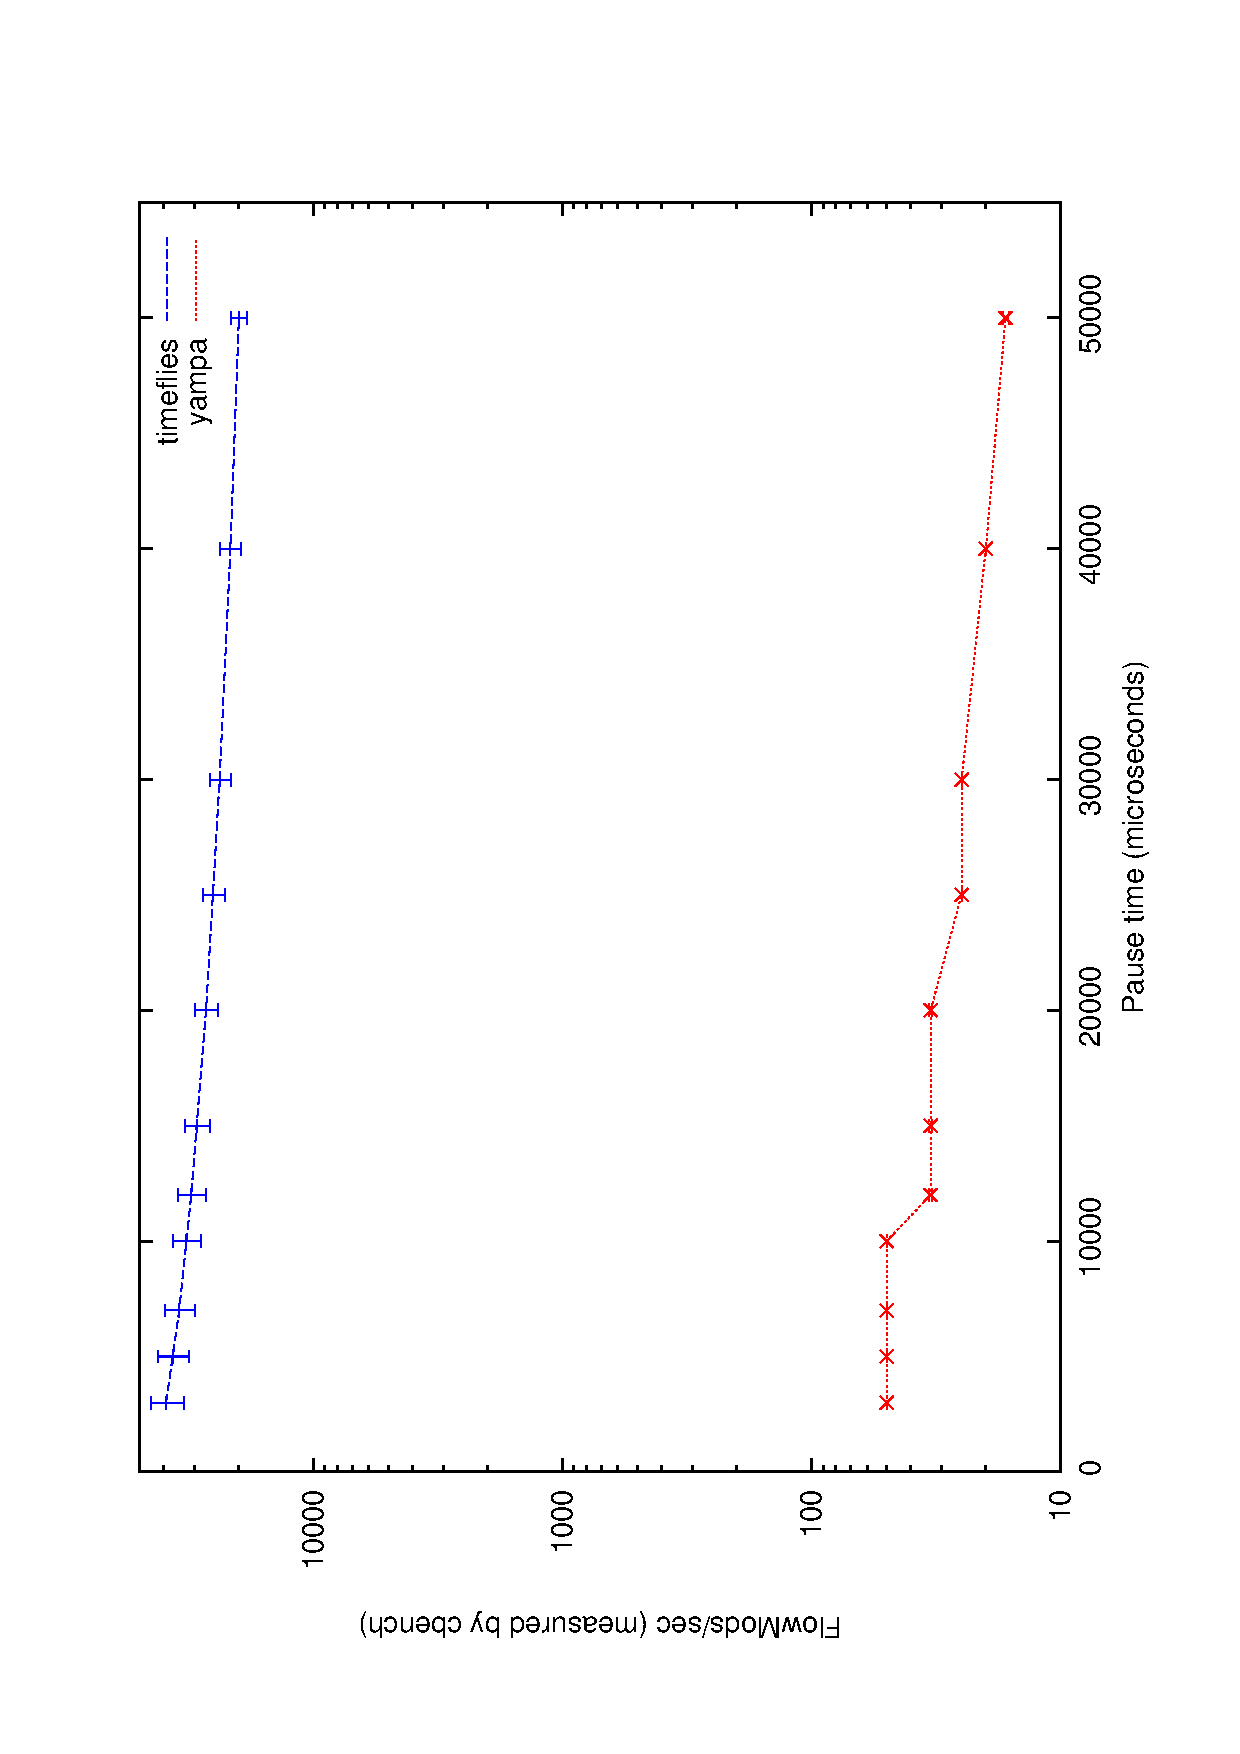
\includegraphics{graph}
\hrule
\caption{Comparison of timeflies vs. Yampa implementing an OpenFlow learning switch controller.}
\label{fig:timeflies-yampa-comparison}
\end{figure}

There is some correlation between the sampling rate and the response rate
for TimeFlies, which is due to the continued wrapping of a replacement signal
function by {\tt switch} until the next time step (see Section~\ref{subsection:Implementation-Signal_Functions-Implementation_of_Signal_Function_Combinators}).
Nevertheless, TimeFlies outperforms Yampa in event response by several orders of magnitude,
even at a very high sampling rate. This is due to two factors. First, TimeFlies can react
to individual events without evaluating the whole signal function. Second, in
the implementation described in Chapter~\ref{chapter:Example_Application}, the
interface of TimeFlies permits us to connect its evaluation directly to GHC's
event manager, while the design of Yampa requires us to use threads and
synchronized communication\footnote{Yampa does include a step-wise evaluation
function, but it still couples event evaluation firmly to time steps, and is not well
documented.}. Even the TimeFlies implementation using polling IO outperforms the
Yampa version, due to the ability to evaluate multiple events per time step.

